\documentclass[11pt,a4paper]{article}
\usepackage[T1]{fontenc}
\usepackage[utf8]{inputenc}
\usepackage{lmodern}
\usepackage{microtype}
\usepackage[margin=2.5cm]{geometry}
\usepackage{amsmath,amssymb}
\usepackage{graphicx}
\usepackage{booktabs}
\usepackage{caption}
\usepackage{float}
\usepackage{setspace}
\usepackage[authoryear,round]{natbib}
\usepackage{xcolor}
\usepackage[colorlinks=true,linkcolor=blue!50!black,citecolor=blue!50!black,urlcolor=blue!50!black]{hyperref}
\usepackage{threeparttable}
\usepackage{enumitem}
\captionsetup{font=small,labelfont=bf,margin=0.5cm}
\setstretch{1.12}
\setlength{\parskip}{0.35em}
\newcommand{\figwidth}{\textwidth}
\graphicspath{{figures/}}

\title{\textbf{Oil Shocks, Inflation Pass-Through and the Pricing of Inflation Risk}\\[0.3em]
\large Evidence from the United States and the Euro Area, 1990--2026}
\author{[Group members]\\[0.2em] \small Macro \& Capital Markets --- Group project}
\date{November 2026}

\begin{document}
\maketitle

\begin{abstract}
\noindent We measure how much and how quickly oil price movements pass through to realized inflation in the United States and the euro area, and whether market-based inflation expectations react in a way consistent with that pass-through. Using local projections on monthly data for 1990--2026, we find that a 10\% rise in Brent raises headline inflation by about 0.55 pp in the US and 0.4--0.5 pp in the euro area within 6--12 months, but core inflation by only 0.1--0.2 pp. Pass-through to core was close to zero before 2020 and rose markedly afterwards. On the market side, weekly regressions show that 5-year inflation compensation rises by 5--7 bp per 10\% oil move, while the 5y5y forward barely moves except during 2021--23. Separating oil shocks with sign and narrative restrictions reveals that the market response depends on the cause of the oil move: oil-specific (supply) shocks leave long-term expectations unchanged, whereas oil rises driven by global demand move the 5y5y forward by 6--13 bp. Finally, a model estimated only on 1990--2019 data accurately predicts US inflation after the record oil shock of March 2026, attributing about 1.1 pp of it to oil, which supports the markets' decision to treat that shock as temporary.
\end{abstract}

\vspace{0.5em}
\noindent\textbf{Keywords:} oil shocks, inflation pass-through, breakeven inflation, inflation swaps, local projections, anchoring of expectations.

\section{Introduction}

An oil price shock is first a cash-flow shock: it raises firms' production costs and households' consumer prices. Whether it also becomes a discount-rate shock, moving interest rates and asset prices, depends on how investors read it. If the shock is expected to be temporary, it should affect inflation for a few months and leave long-term inflation expectations unchanged. If investors fear second-round effects through wages and core prices, long-term expectations rise, and with them the risk that central banks must tighten. Whether long-term inflation expectations stay \emph{anchored} after energy shocks is therefore a central question for monetary policy and for the pricing of bonds and inflation-linked assets.

This paper asks two connected questions. First, when oil prices move, how much and how fast does the move show up in realized headline and core inflation in the US and the euro area? Second, do market inflation expectations, measured by breakeven inflation rates and inflation swaps, react in a way that is consistent with that realized pass-through? We test four hypotheses:
\begin{enumerate}[label=\textbf{H\arabic*.},leftmargin=2.2em,itemsep=0.1em]
\item Oil passes through strongly and quickly to headline inflation, but only weakly and with a lag to core inflation.
\item Pass-through is stronger in the euro area than in the US, because the euro area imports most of its energy.
\item Short-term market expectations (5-year) react to oil, but long-term expectations (5y5y forward) barely move: markets treat oil shocks as temporary.
\item Pass-through has changed over time, and was larger after 2020.
\end{enumerate}

Our sample includes an unusually informative episode. In March 2026 the war involving Iran disrupted oil flows through the Strait of Hormuz, and Brent recorded its largest monthly gain on record \citep{reuters2026}. Because this shock occurs after the end of our main estimation sample, it provides a genuine out-of-sample test of the estimated pass-through and of the markets' reading of the shock.

Our main contributions are threefold. (i) We document pass-through jointly for realized inflation and for market expectations across the term structure, for both regions, with the same shock measure. (ii) We show that the market reaction depends on \emph{why} oil moves: separating oil-specific from demand-driven oil movements resolves much of the variation in the sensitivity of long-term expectations. (iii) We test the estimated pass-through out of sample on the 2026 shock.

\section{Related literature}

A large literature studies the macroeconomic effects of oil price shocks. \citet{hooker2002} documents that pass-through of oil prices to US core inflation declined sharply after the early 1980s, and \citet{blanchard2010} attribute the milder effects of oil shocks in the 2000s to smaller energy shares, more flexible labour markets and more credible monetary policy. Several papers stress that oil price increases and decreases may have asymmetric effects \citep{mork1989}, and that retail fuel prices rise faster than they fall \citep{peltzman2000}.

A second strand emphasizes that not all oil price shocks are alike. \citet{kilian2009} separates oil supply shocks, global demand shocks and oil-specific (precautionary) demand shocks in a structural VAR, and \citet{baumeister2019} revisit this decomposition with Bayesian priors on elasticities. \citet{kanzig2021} identifies oil supply news shocks from futures price movements around OPEC announcements. Closest to our identification strategy, \citet{kilianpark2009} and \citet{ready2018} use the co-movement of oil and stock prices to separate demand from supply shocks: demand shocks raise both oil and equity prices, whereas supply shocks raise oil prices but lower equity prices. We implement this idea with sign restrictions \citep{uhlig2005} sharpened by narrative restrictions \citep{antolin2018}.

A third strand studies inflation expectations. \citet{coibion2015} show that household inflation expectations are highly sensitive to oil and gasoline prices, and \citet{kilianzhou2022} analyze the link between gasoline prices and expectations. On the market side, \citet{gurkaynak2005} document an ``excess sensitivity'' of long-term forward rates to macroeconomic news, which is a sign of imperfectly anchored expectations. Market measures of inflation compensation also contain inflation risk and liquidity premia \citep{damico2018}, a caveat we return to below. Methodologically, we rely on local projections \citep{jorda2005} with heteroskedasticity- and autocorrelation-robust standard errors \citep{newey1987}.

\section{Data}

All series are downloaded from Bloomberg. Table~\ref{tab:data} summarizes them.

\begin{table}[!htbp]
\centering\small
\caption{Data}\label{tab:data}
\begin{minipage}{\textwidth}\centering
\resizebox{\textwidth}{!}{\begin{tabular}{llll}
\toprule
Variable & Ticker & Frequency & Sample\\
\midrule
Brent crude, front month & CO1 Comdty & Monthly, daily & 1990--2026; 2004--2026\\
WTI crude, front month & CL1 Comdty & Monthly, daily & 1990--2026; 2004--2026\\
Bloomberg Commodity Index & BCOM Index & Monthly & 1990--2026\\
US CPI, headline and core (YoY) & CPI YOY, CPI XYOY & Monthly & 1990--Sep 2026\\
US CPI index (NSA) & CPURNSA & Monthly & 1990--Oct 2026\\
Euro area HICP, headline and core (YoY) & ECCPEMUY, CPEXEMUY & Monthly & 1997--Oct 2026\\
Euro area HICP index & CPTFEMU & Monthly & 1996--Sep 2026\\
US 5-year breakeven inflation & USGGBE05 & Daily & 2004--2026\\
US 5y5y inflation swap forward & FWISUS55 & Daily & 2004--2026\\
Euro area 5-year inflation swap & EUSWI5 & Daily & 2004--2026\\
Euro area 5y5y inflation swap forward & FWISEU55 & Daily & 2004--2026\\
S\&P 500 & SPX Index & Daily & 2004--2026\\
\bottomrule
\end{tabular}}
\par\smallskip{\footnotesize\raggedright \textit{Notes:} Inflation regressions use monthly data; market regressions use weekly (Friday) changes built from daily closes. Daily data end on 17 November 2026.\par}
\end{minipage}
\end{table}

\paragraph{Oil price measure.} Consumer prices are measured as averages over the month, so the relevant oil price is the monthly \emph{average} Brent price. From 2004 we compute it from daily closes. Before 2004, when only month-end prices are available, we approximate it by the geometric mean of adjacent month-end prices (correlation 0.87 with the true average over 2004--2026). The shock is the monthly log change of this average, $o_t = 100\,\Delta\ln(\text{Brent}_t)$. We use nominal Brent in US dollars: deflating by the CPI changes the estimates by at most 0.03 pp, and would put the dependent variable on both sides of the regression. Brent is preferred to WTI because WTI closed at a negative price on 20 April 2020.

\paragraph{Data adjustments.} The US CPI for October 2025 was never published because of the federal government shutdown; we fill this single month by linear interpolation. The euro area HICP series starts in December 1996, so euro area regressions start in 1997.

\section{Methodology}

\subsection{Inflation pass-through: local projections}
Let $\pi_t$ denote year-on-year inflation (headline or core) in percent. For each horizon $h=0,\dots,24$ months we estimate
\begin{equation}
\pi_{t+h}-\pi_{t-1} = \alpha_h + \beta_h\, o_t + \sum_{j=1}^{6}\left(\gamma_{h,j}\, o_{t-j} + \delta_{h,j}\,\Delta\pi_{t-j}\right) + \varepsilon_{t+h},
\label{eq:lp}
\end{equation}
with Newey--West standard errors using $h+1$ lags. The sequence $\{10\,\beta_h\}_{h=0}^{24}$ traces the cumulative response of YoY inflation (in percentage points) to a 10\% rise in Brent. Because inflation is measured year-on-year, the response of a one-time oil price level shift naturally declines after 12 months as the shock drops out of the annual comparison (the base effect). We estimate (\ref{eq:lp}) on the full sample, before 2020 and from 2020 onwards. Replacing $\pi_t$ by $100\ln P_t$ (the log price index, with monthly seasonal dummies) gives the response of the price \emph{level}, which we use in Section~\ref{sec:consistency}.

\subsection{Market reaction}
For each measure of inflation compensation $x_t$ (5-year and 5y5y, US and euro area) we estimate on weekly data
\begin{equation}
\Delta x_t = a + b\, o^{w}_t + c\, r^{SPX}_t + u_t,
\label{eq:mkt}
\end{equation}
where $\Delta x_t$ is the weekly change in basis points, $o^w_t$ the weekly Brent log return and $r^{SPX}_t$ the S\&P 500 log return, which controls for broad risk-on/risk-off moves. We report $10\,b$, the move in basis points per 10\% oil move. Weekly rather than daily data avoid problems from different closing times across markets; we also report daily and monthly estimates.

\subsection{Global-demand versus oil-specific shocks}
Let $u_t=(o^w_t, r^{SPX}_t)'$ denote demeaned weekly returns with covariance $\Sigma = PP'$, where $P$ is the Cholesky factor. We write $u_t = A\,\varepsilon_t$ with $A = P\,Q(\theta)$ and $Q(\theta)$ a rotation matrix. We impose:
\begin{itemize}[itemsep=0.1em]
\item \textbf{Sign restrictions.} A \emph{global-demand} shock raises both oil and stock prices on impact; an \emph{oil-specific} shock (supply disruptions and precautionary demand) raises oil prices and lowers stock prices.
\item \textbf{Narrative restrictions.} In four weeks whose cause is well documented, the named shock has the stated sign and is the main driver of the oil move: the post-Lehman collapse (week of 10 October 2008: negative demand shock), the Saudi--Russian price war (13 March 2020: negative oil-specific shock), Russia's invasion of Ukraine (4 March 2022: positive oil-specific shock), and the outbreak of the war involving Iran (6 March 2026: positive oil-specific shock).
\end{itemize}
Sign restrictions alone are consistent with any share of oil variance being oil-specific; the narrative restrictions narrow the admissible set to rotations attributing 69--92\% of weekly oil variance to oil-specific shocks. Our baseline uses the midpoint of the admissible set (82\%), and we report results at both ends. The oil return is then split into a demand-driven and an oil-specific component, which replace $o^w_t$ in (\ref{eq:mkt}). Monthly sums of the two components replace $o_t$ in (\ref{eq:lp}) over 2005--2026.

\subsection{Out-of-sample test on the 2026 shock}
We estimate a distributed-lag model for the monthly change in YoY inflation,
\begin{equation}
\Delta\pi_t = c + \sum_{j=0}^{13} b_j\, o_{t-j} + \sum_{j=1}^{13} g_j\, \Delta\pi_{t-j} + e_t,
\label{eq:ardl}
\end{equation}
where 13 lags of oil capture the base effect after one year. The model is estimated on 1990--2019 and, alternatively, on 1990--February 2026. Starting from actual inflation in February 2026, we simulate inflation forward using the \emph{actual} Brent path from March 2026 and the model's own predictions for lagged inflation, never the realized inflation data after February. This is a forecast conditional on the oil path. A counterfactual simulation freezes Brent at its February 2026 level, so the difference between the two isolates the contribution of oil. A 90\% band is obtained from 1{,}000 simulations with bootstrapped residuals.

\section{Results}

\subsection{Pass-through to realized inflation}

Figure~\ref{fig:hc} and Table~\ref{tab:pt} show the main result. A 10\% rise in Brent raises US headline inflation by 0.20 pp in the same month, 0.55 pp after six months and 0.55 pp after a year, with a peak of 0.67 pp after 11 months. The response then falls as the shock leaves the year-on-year comparison. The euro area response is somewhat smaller and slower: 0.42 pp after six months and 0.49 pp after a year. Core inflation responds much less: 0.12 pp (US) and 0.05 pp (euro area) after six months, rising to 0.19 and 0.18 pp after 12--18 months. \textbf{H1 is supported}: oil passes through quickly to headline inflation and only weakly, with a lag, to core.

\textbf{H2 is rejected} for the full sample: pass-through to headline inflation is \emph{larger} in the US than in the euro area. A likely reason is that fuel in Europe is taxed heavily with fixed per-litre excise duties, so a given percentage change in crude prices is a smaller percentage change at the pump. Energy also has a different weight in the two baskets. Since 2020 the ranking has reversed (Figure~\ref{fig:pt}): euro area headline pass-through reaches about 1.1 pp after 12--18 months, against 0.85 pp in the US. This is consistent with the 2022 energy crisis, in which gas prices and a weaker euro amplified the effect of oil in Europe, although our oil-only data cannot separate these channels.

\begin{figure}[!htbp]
\centering
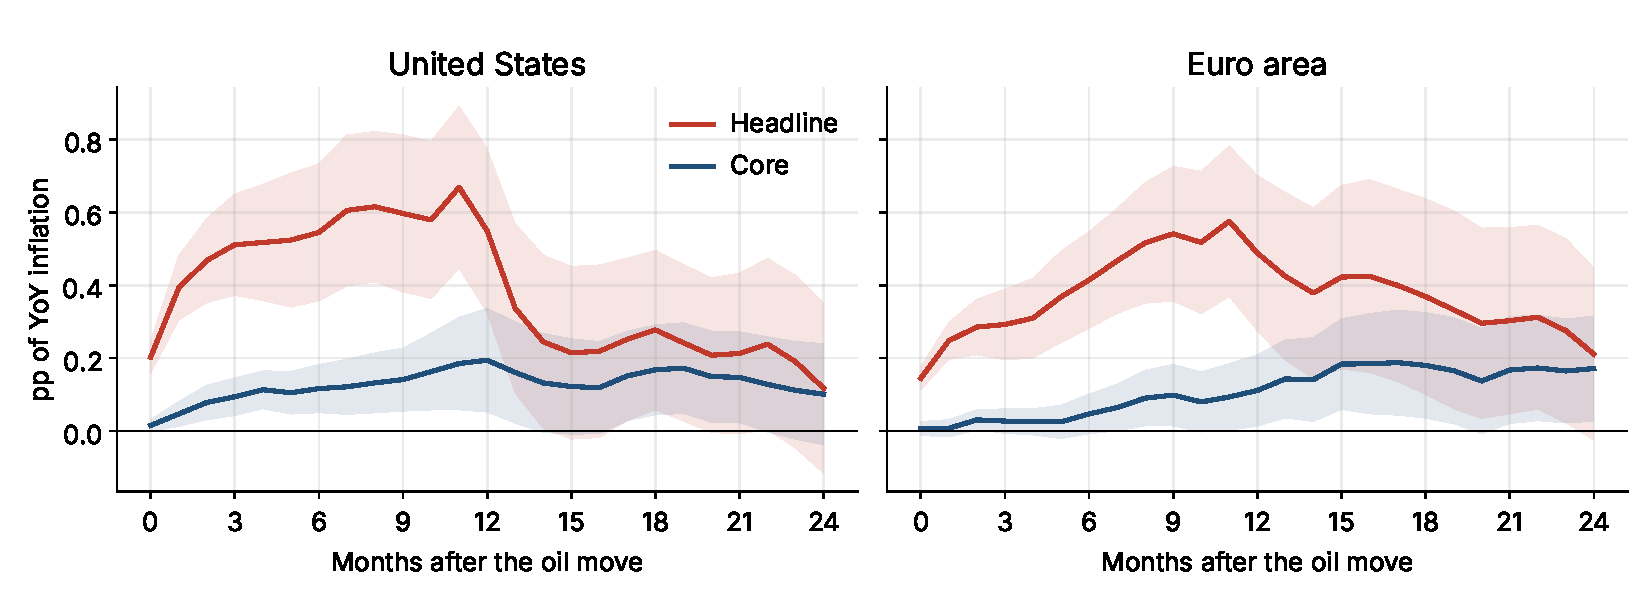
\includegraphics[width=\figwidth]{fig02_headline_vs_core.pdf}
\caption{Response of YoY inflation to a 10\% rise in Brent, headline versus core (1990--2026). Local projections, equation~(\ref{eq:lp}); shaded areas are 90\% confidence bands.}\label{fig:hc}
\end{figure}

\begin{table}[!htbp]
\centering\small
\caption{Pass-through of a 10\% Brent rise to YoY inflation (pp)}\label{tab:pt}
\begin{minipage}{\textwidth}\centering
\begin{tabular}{lrrrrrrr}
\toprule
 & \multicolumn{6}{c}{Months after the oil move ($h$)} & \\ \cmidrule(lr){2-7}
 & 0 & 3 & 6 & 12 & 18 & 24 & Obs.\\
\midrule
\multicolumn{8}{l}{\textit{US headline CPI}}\\
\quad Full sample & 0.20 & 0.51 & 0.55 & 0.55 & 0.28 & 0.12 & 433\\
\quad Pre--2020 & 0.19 & 0.48 & 0.49 & 0.46 & 0.20 & 0.14 & 352\\
\quad 2020--2026 & 0.26 & 0.59 & 0.66 & 0.85 & 0.55 & 0.00 & 81\\
\addlinespace
\multicolumn{8}{l}{\textit{US core CPI}}\\
\quad Full sample & 0.01 & 0.09 & 0.12 & 0.19 & 0.17 & 0.10 & 433\\
\quad Pre--2020 & 0.00 & 0.04 & 0.05 & 0.07 & 0.12 & 0.11 & 352\\
\quad 2020--2026 & 0.08 & 0.27 & 0.31 & 0.68 & 0.45 & 0.09 & 81\\
\addlinespace
\multicolumn{8}{l}{\textit{Euro area headline HICP}}\\
\quad Full sample & 0.14 & 0.29 & 0.41 & 0.49 & 0.37 & 0.21 & 352\\
\quad Pre--2020 & 0.13 & 0.26 & 0.29 & 0.33 & 0.18 & 0.12 & 270\\
\quad 2020--2026 & 0.18 & 0.42 & 0.78 & 1.07 & 1.07 & 0.57 & 82\\
\addlinespace
\multicolumn{8}{l}{\textit{Euro area core HICP}}\\
\quad Full sample & 0.01 & 0.03 & 0.05 & 0.11 & 0.18 & 0.17 & 352\\
\quad Pre--2020 & 0.00 & 0.02 & 0.00 & 0.03 & 0.07 & 0.09 & 270\\
\quad 2020--2026 & $-$0.01 & 0.04 & 0.16 & 0.40 & 0.55 & 0.47 & 82\\
\bottomrule
\end{tabular}
\par\smallskip{\footnotesize\raggedright \textit{Notes:} Coefficients $10\beta_h$ from equation~(\ref{eq:lp}). Full-sample 90\% confidence bands are shown in Figures~\ref{fig:hc}--\ref{fig:pt}. Typical standard errors at $h=6$: 0.11 (US headline), 0.04 (US core), 0.08 (EA headline), 0.03 (EA core).\par}
\end{minipage}
\end{table}

\textbf{H4 is supported, mainly for core inflation.} Before 2020, pass-through to core was essentially zero (0.07 pp in the US and 0.03 pp in the euro area after a year), in line with \citet{hooker2002}. Since 2020 it is substantial: 0.68 pp in the US after 12 months and 0.40--0.55 pp in the euro area after 12--18 months (Figure~\ref{fig:pt}). Two caveats apply. The post-2020 sample has only about 80 monthly observations, and in 2021--22 oil prices rose together with the post-pandemic recovery and supply-chain disruptions, so part of this estimate likely reflects those common factors rather than oil alone.

\begin{figure}[!htbp]
\centering
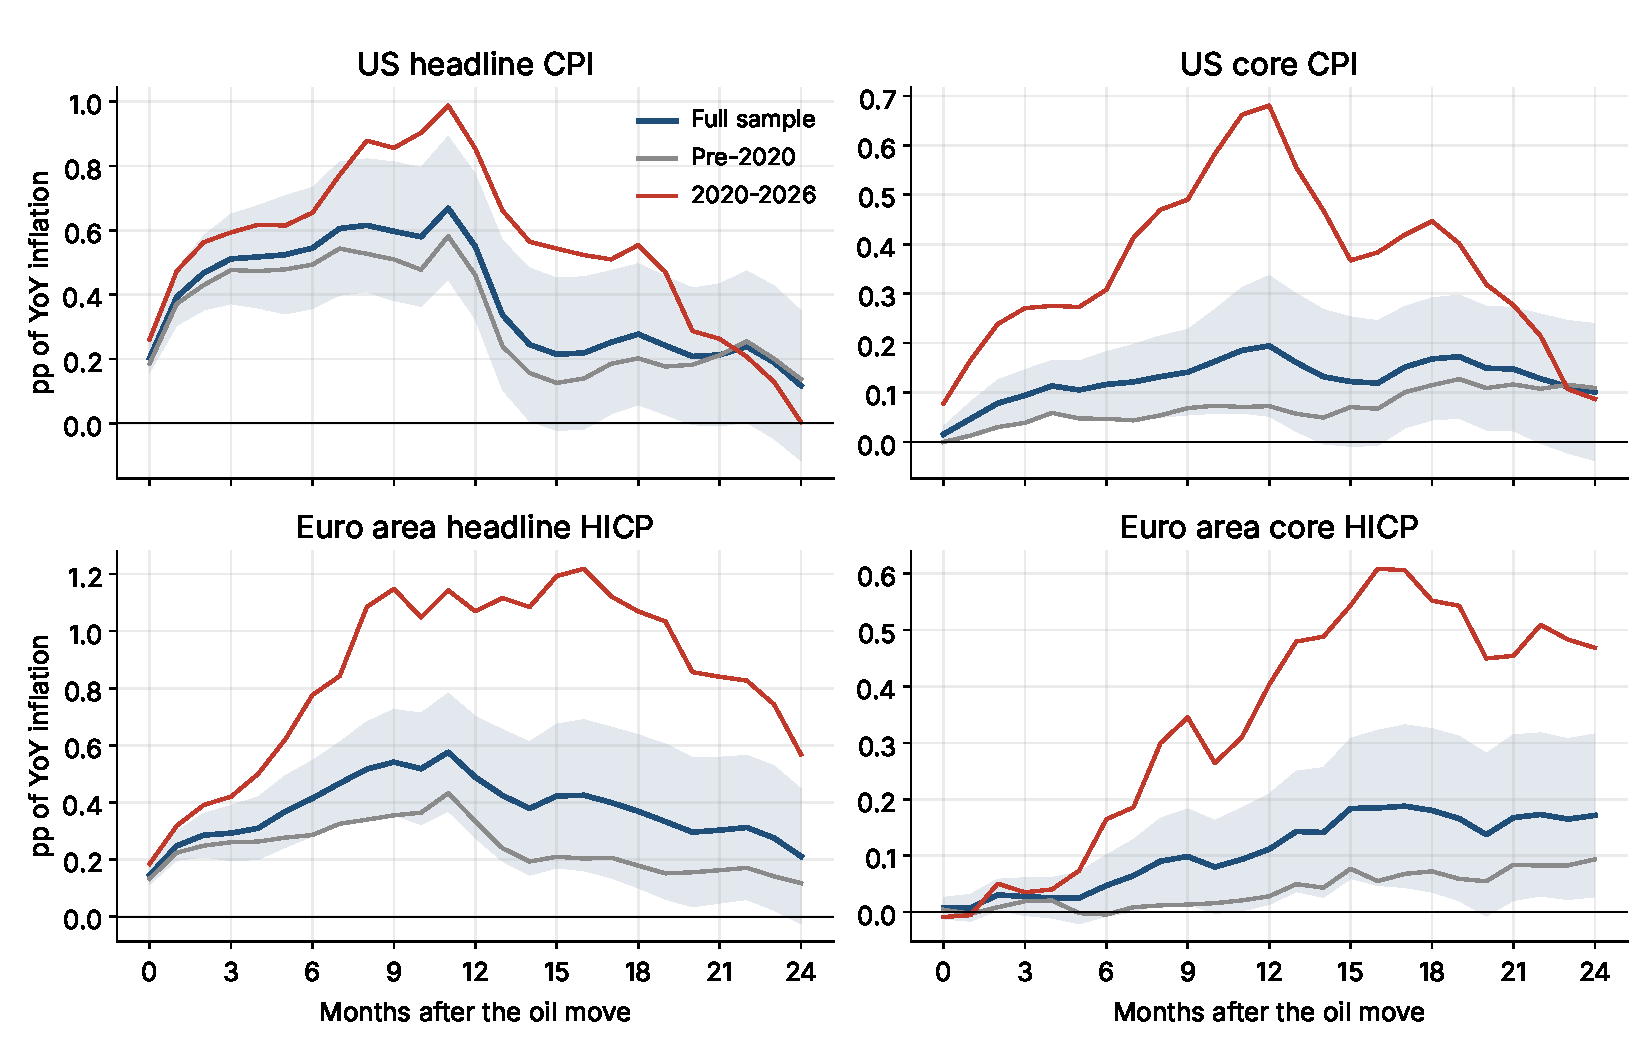
\includegraphics[width=\figwidth]{fig01_passthrough_by_sample.pdf}
\caption{Pass-through before and after 2020. Response of YoY inflation to a 10\% rise in Brent; the 90\% band refers to the full sample.}\label{fig:pt}
\end{figure}

\subsection{Market inflation expectations}

Table~\ref{tab:mkt} and Figure~\ref{fig:mkt} report the sensitivity of inflation compensation to oil. Over 2004--2026, a 10\% rise in Brent raises the US 5-year breakeven by 6.8 bp and the euro area 5-year swap by 5.4 bp, both highly significant. The 5y5y forward barely moves: $-0.4$ bp in the US (not significant) and $+1.2$ bp in the euro area. \textbf{H3 is supported on average}: markets price oil into inflation over the next five years, but not into long-term expectations.

The exception is 2021--2023, when both 5y5y forwards rose by about 4 bp per 10\% oil move, and short-term sensitivities roughly doubled to 12 bp. This is the period in which inflation was high and central banks were widely seen as behind the curve. Rolling two-year estimates (Figure~\ref{fig:roll} in the Appendix) confirm that long-term sensitivity is close to zero for most of the sample and peaks in 2022. After the March 2026 shock, short-term sensitivity is high in the euro area (11 bp) but the 5y5y response remains small (1--2 bp).

\begin{table}[!htbp]
\centering\small
\caption{Sensitivity of inflation compensation to a 10\% Brent move (bp, weekly)}\label{tab:mkt}
\begin{minipage}{\textwidth}\centering
\begin{tabular}{lrrrrr}
\toprule
 & \multicolumn{2}{c}{United States} & \multicolumn{2}{c}{Euro area} & \\ \cmidrule(lr){2-3}\cmidrule(lr){4-5}
Period & 5y BEI & 5y5y swap & 5y swap & 5y5y swap & Weeks\\
\midrule
2004--2026 & $6.80^{***}$ & $-0.37$ & $5.40^{***}$ & $1.17^{**}$ & 1194\\
 & {\footnotesize (0.96)} & {\footnotesize (1.51)} & {\footnotesize (0.75)} & {\footnotesize (0.46)} & \\
\midrule
2004--2008 & $5.93^{*}$ & $-5.09$ & $2.64^{*}$ & $-0.34$ & 260\\
 & {\footnotesize (3.37)} & {\footnotesize (5.64)} & {\footnotesize (1.57)} & {\footnotesize (1.22)} & \\
2009--2019 & $6.31^{***}$ & $0.91$ & $2.93^{***}$ & $-0.15$ & 574\\
 & {\footnotesize (0.75)} & {\footnotesize (1.16)} & {\footnotesize (0.67)} & {\footnotesize (0.62)} & \\
2020 & $4.50^{**}$ & $-3.05^{*}$ & $2.94^{***}$ & $1.21^{***}$ & 52\\
 & {\footnotesize (1.91)} & {\footnotesize (1.73)} & {\footnotesize (0.65)} & {\footnotesize (0.44)} & \\
2021--2023 & $11.87^{***}$ & $3.81^{***}$ & $12.04^{***}$ & $4.04^{***}$ & 157\\
 & {\footnotesize (1.14)} & {\footnotesize (1.12)} & {\footnotesize (2.29)} & {\footnotesize (1.31)} & \\
2024--2026 & $6.79^{***}$ & $1.74^{***}$ & $9.09^{***}$ & $1.78^{***}$ & 151\\
 & {\footnotesize (0.85)} & {\footnotesize (0.44)} & {\footnotesize (0.91)} & {\footnotesize (0.38)} & \\
Iran shock (Mar--Nov 2026) & $6.17^{***}$ & $1.25^{**}$ & $11.40^{***}$ & $2.05^{***}$ & 39\\
 & {\footnotesize (1.08)} & {\footnotesize (0.49)} & {\footnotesize (0.96)} & {\footnotesize (0.39)} & \\
\bottomrule
\end{tabular}
\par\smallskip{\footnotesize\raggedright \textit{Notes:} Coefficient $10b$ from equation~(\ref{eq:mkt}), controlling for the S\&P 500 return. Newey--West standard errors (4 lags) in parentheses. $^{*}$, $^{**}$, $^{***}$: significant at 10\%, 5\%, 1\%.\par}
\end{minipage}
\end{table}

\begin{figure}[!htbp]
\centering
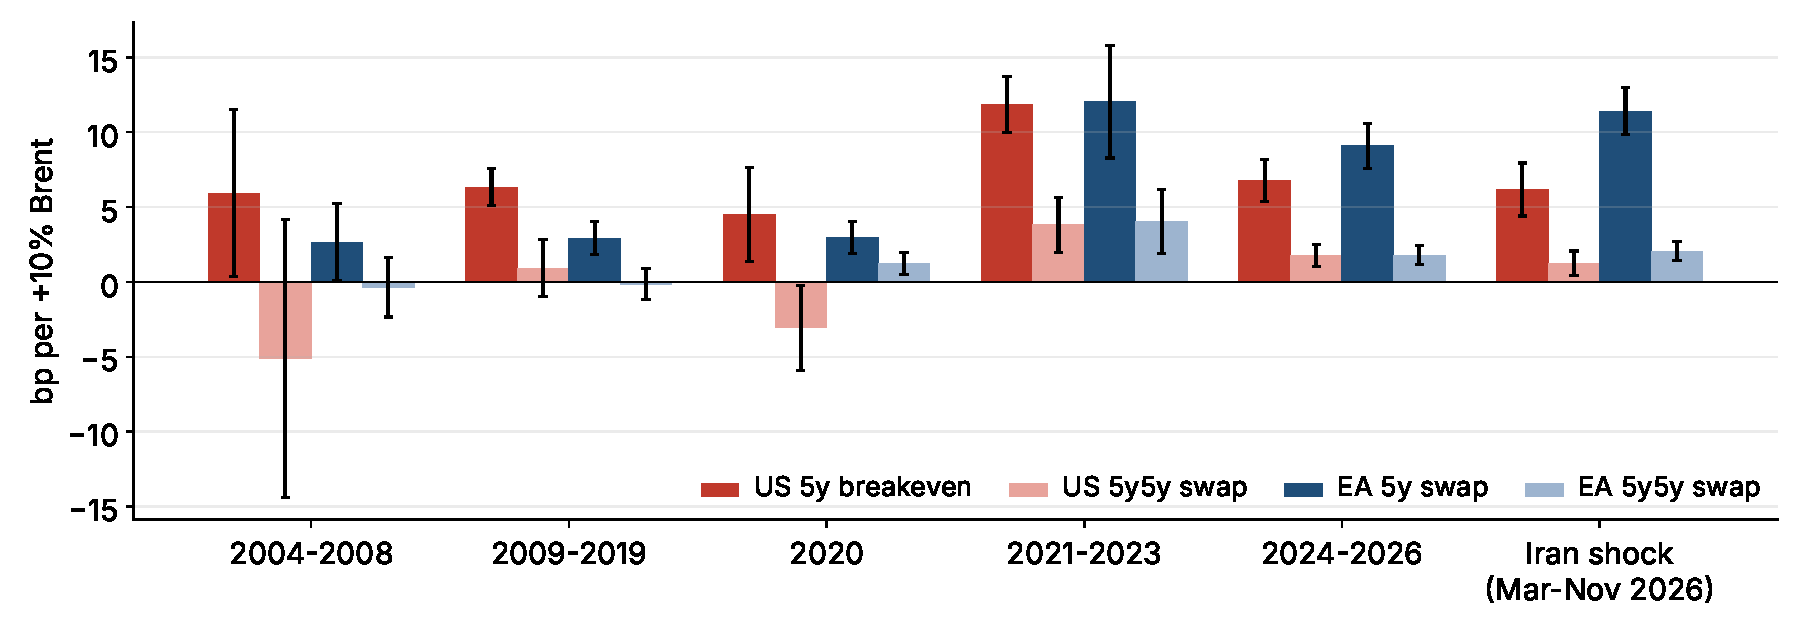
\includegraphics[width=\figwidth]{fig04_market_betas_by_period.pdf}
\caption{Sensitivity of 5-year and 5y5y inflation compensation to a 10\% Brent move, by period (weekly regressions with S\&P 500 control, 90\% confidence intervals).}\label{fig:mkt}
\end{figure}

\paragraph{2022 versus 2026.} Figure~\ref{fig:episodes} and Table~\ref{tab:episodes} compare the two largest recent oil supply shocks. In 2022, a 32\% rise in Brent after Russia's invasion of Ukraine was accompanied by a rise of 33--39 bp in the 5y5y forwards. In 2026, a much larger 63\% rise was accompanied by changes of only $-5$ bp (US) and $+5$ bp (euro area) in the 5y5y. Short-term expectations rose in both episodes. Markets therefore treated the 2026 shock as temporary, while in 2022 they priced a risk of de-anchoring. The 2022 episode also involved a gas price shock in Europe and a monetary policy stance perceived as too loose, so the contrast should not be attributed to oil alone.

\begin{figure}[!htbp]
\centering
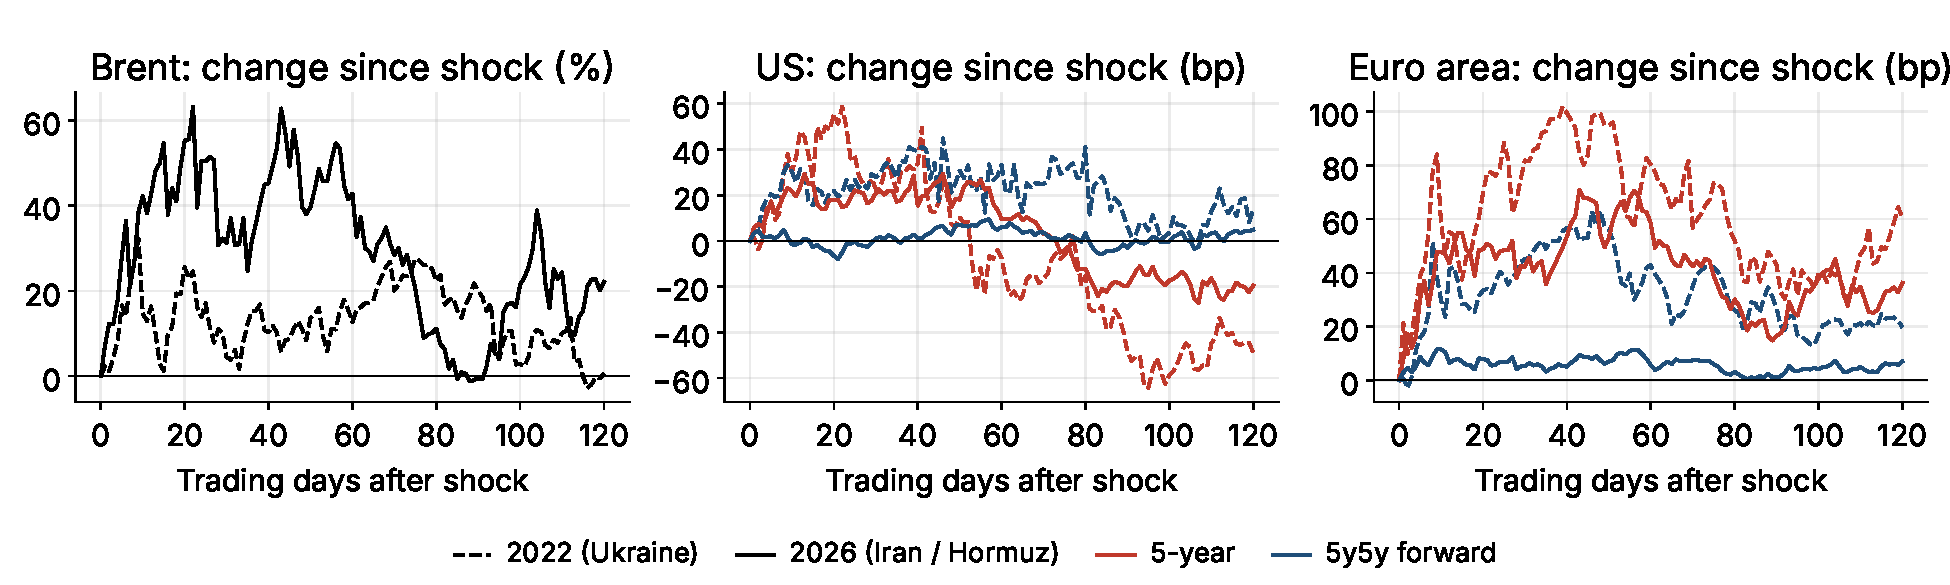
\includegraphics[width=\figwidth]{fig05_2022_vs_2026.pdf}
\caption{Brent and inflation compensation after the 2022 and 2026 oil supply shocks (dashed: from 23 February 2022; solid: from 27 February 2026).}\label{fig:episodes}
\end{figure}

\begin{table}[!htbp]
\centering\small
\caption{Two oil supply shocks: changes from the day before the shock}\label{tab:episodes}
\begin{tabular}{lrrrrr}
\toprule
 & Brent & \multicolumn{2}{c}{United States (bp)} & \multicolumn{2}{c}{Euro area (bp)}\\ \cmidrule(lr){3-4}\cmidrule(lr){5-6}
Episode & peak (\%) & 5y BEI & 5y5y & 5y & 5y5y\\
\midrule
2022 (Ukraine) & 32.2 & 37.9 & 33.1 & 84.1 & 38.5\\
\quad max.\ move within 120 days & & 58.7 & 44.9 & 101.9 & 63.1\\
2026 (Iran /  Hormuz) & 63.3 & 14.7 & $-$5.0 & 49.7 & 5.4\\
\quad max.\ move within 120 days & & 29.3 & 9.5 & 70.9 & 11.6\\
\bottomrule
\end{tabular}
\end{table}

\subsection{Are markets consistent with realized pass-through?}\label{sec:consistency}

To compare the two halves of the analysis we translate realized pass-through into an implied change in average inflation over five years. The price-level local projection implies that a 10\% Brent rise raises the US price level by 0.59\% and the euro area price level by 0.65\% after 24 months. If there is no further effect in years three to five, average annual inflation over five years rises by roughly one fifth of that, i.e.\ 12--13 bp. Table~\ref{tab:cons} compares this with the observed 5-year market moves.

\begin{table}[!htbp]
\centering\small
\caption{Realized pass-through versus market pricing (per 10\% Brent rise)}\label{tab:cons}
\begin{tabular}{lrrrrr}
\toprule
 & \multicolumn{2}{c}{Price-level effect (\%)} & Implied 5y avg. & Observed 5y & \\ \cmidrule(lr){2-3}
Region & 12 months & 24 months & inflation (bp) & market move (bp) & Ratio\\
\midrule
US & 0.60 & 0.59 & 11.8 & 6.8 & 0.57\\
Euro area & 0.55 & 0.65 & 13.0 & 5.4 & 0.41\\
\bottomrule
\end{tabular}
\end{table}

Weekly market moves correspond to roughly 60\% (US) and 40\% (euro area) of the implied effect. With monthly market data the sensitivities are larger (9.7 and 7.8 bp; Table~\ref{tab:robmkt}), raising the ratios to about 80\% and 60\%. Markets therefore price most of the realized effect in the US and somewhat less in the euro area. This comparison is only indicative: it assumes the oil move is permanent, ignores effects beyond two years, and treats inflation compensation as pure expected inflation, whereas it also contains risk and liquidity premia.

\subsection{Why the oil move matters: demand versus oil-specific shocks}

Figure~\ref{fig:decomp} shows the historical decomposition of weekly oil returns. The identification attributes the 2014--15 collapse (after OPEC's decision not to cut output), the March 2022 surge and the March 2026 surge almost entirely to oil-specific factors, and about one third of the late-2008 collapse to falling global demand. The baseline attributes 82\% of weekly oil variance to oil-specific shocks, which is high relative to VAR-based studies. In particular, the stock-based identification classifies most of the 2004--08 run-up and much of the late-2008 collapse as oil-specific, whereas VAR-based identifications \citep{kilian2009} attribute both largely to global demand. Because oil-specific shocks are identified as moves in oil \emph{not} matched by equity prices, we view this split as conservative for our main result: any demand shocks misclassified as oil-specific would bias the oil-specific response of expectations upward, not downward.

\begin{figure}[!htbp]
\centering
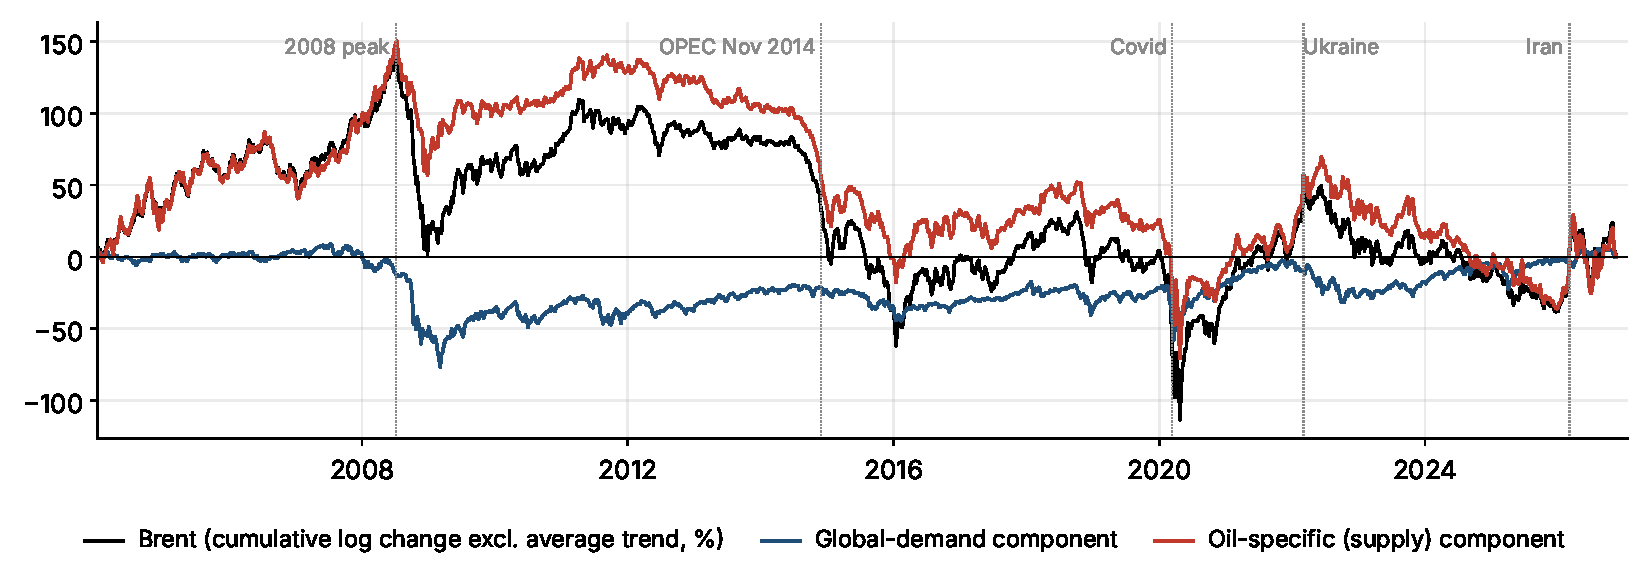
\includegraphics[width=\figwidth]{fig07_oil_shock_decomposition.pdf}
\caption{Historical decomposition of weekly Brent returns into global-demand and oil-specific components (cumulative, excluding the average trend), using sign and narrative restrictions.}\label{fig:decomp}
\end{figure}

Table~\ref{tab:shock} and Figure~\ref{fig:shockmkt} contain the main new result. \textbf{The response of long-term expectations depends on the cause of the oil move.} An oil-specific rise of 10\% leaves the 5y5y forward unchanged ($-1.3$ bp in the US, $+0.9$ bp in the euro area), while a demand-driven rise of 10\% raises it by 13.1 bp in the US and 5.6 bp in the euro area. Short-term expectations respond to both, but about three times more to demand-driven moves in the US. The pattern holds before and after 2020 and across all admissible identifications: the US 5y5y response ranges between 9.6 and 20.0 bp for demand-driven moves and between $-2.4$ and $-0.4$ bp for oil-specific moves.

\begin{table}[!htbp]
\centering\small
\caption{Sensitivity of inflation compensation by type of oil shock (bp per 10\% Brent move, weekly)}\label{tab:shock}
\begin{minipage}{\textwidth}\centering
\begin{tabular}{lrrrr}
\toprule
 & \multicolumn{2}{c}{United States} & \multicolumn{2}{c}{Euro area} \\ \cmidrule(lr){2-3}\cmidrule(lr){4-5}
 & 5y BEI & 5y5y swap & 5y swap & 5y5y swap\\
\midrule
\multicolumn{5}{l}{\textit{2004--2026}}\\
\quad Global-demand-driven oil rise & $20.66^{***}$ & $13.13^{***}$ & $9.21^{***}$ & $5.61^{***}$\\
 & {\footnotesize (2.12)} & {\footnotesize (2.07)} & {\footnotesize (1.93)} & {\footnotesize (1.24)}\\
\quad Oil-specific (supply) rise & $5.81^{***}$ & $-1.33$ & $5.12^{***}$ & $0.86^{*}$\\
 & {\footnotesize (0.96)} & {\footnotesize (1.63)} & {\footnotesize (0.78)} & {\footnotesize (0.47)}\\
\addlinespace
\multicolumn{5}{l}{\textit{2004--2019}}\\
\quad Global-demand-driven oil rise & $21.39^{***}$ & $15.24^{***}$ & $6.75^{***}$ & $5.07^{***}$\\
 & {\footnotesize (2.98)} & {\footnotesize (2.95)} & {\footnotesize (2.53)} & {\footnotesize (1.56)}\\
\quad Oil-specific (supply) rise & $5.04^{***}$ & $-2.81$ & $2.78^{***}$ & $-0.43$\\
 & {\footnotesize (1.54)} & {\footnotesize (2.97)} & {\footnotesize (0.72)} & {\footnotesize (0.66)}\\
\addlinespace
\multicolumn{5}{l}{\textit{2020--2026}}\\
\quad Global-demand-driven oil rise & $19.35^{***}$ & $9.47^{***}$ & $13.49^{***}$ & $6.52^{***}$\\
 & {\footnotesize (2.40)} & {\footnotesize (1.78)} & {\footnotesize (1.80)} & {\footnotesize (1.75)}\\
\quad Oil-specific (supply) rise & $6.64^{***}$ & $0.15$ & $7.56^{***}$ & $2.20^{***}$\\
 & {\footnotesize (1.15)} & {\footnotesize (1.35)} & {\footnotesize (1.52)} & {\footnotesize (0.63)}\\
\addlinespace
\midrule
\multicolumn{5}{l}{\textit{Range across admissible identifications, 2004--2026}}\\
\quad Global-demand-driven & [17.0, 27.7] & [9.6, 20.0] & [8.2, 11.2] & [4.4, 7.9]\\
\quad Oil-specific (supply) & [4.7, 6.8] & [$-$2.4, $-$0.4] & [4.8, 5.4] & [0.5, 1.2]\\
\bottomrule
\end{tabular}
\par\smallskip{\footnotesize\raggedright \textit{Notes:} Weekly changes regressed on the demand-driven and oil-specific components of the Brent return. Newey--West standard errors (4 lags) in parentheses. The last panel reports the range of point estimates at the two ends of the set of identifications admitted by the sign and narrative restrictions.\par}
\end{minipage}
\end{table}

\begin{figure}[!htbp]
\centering
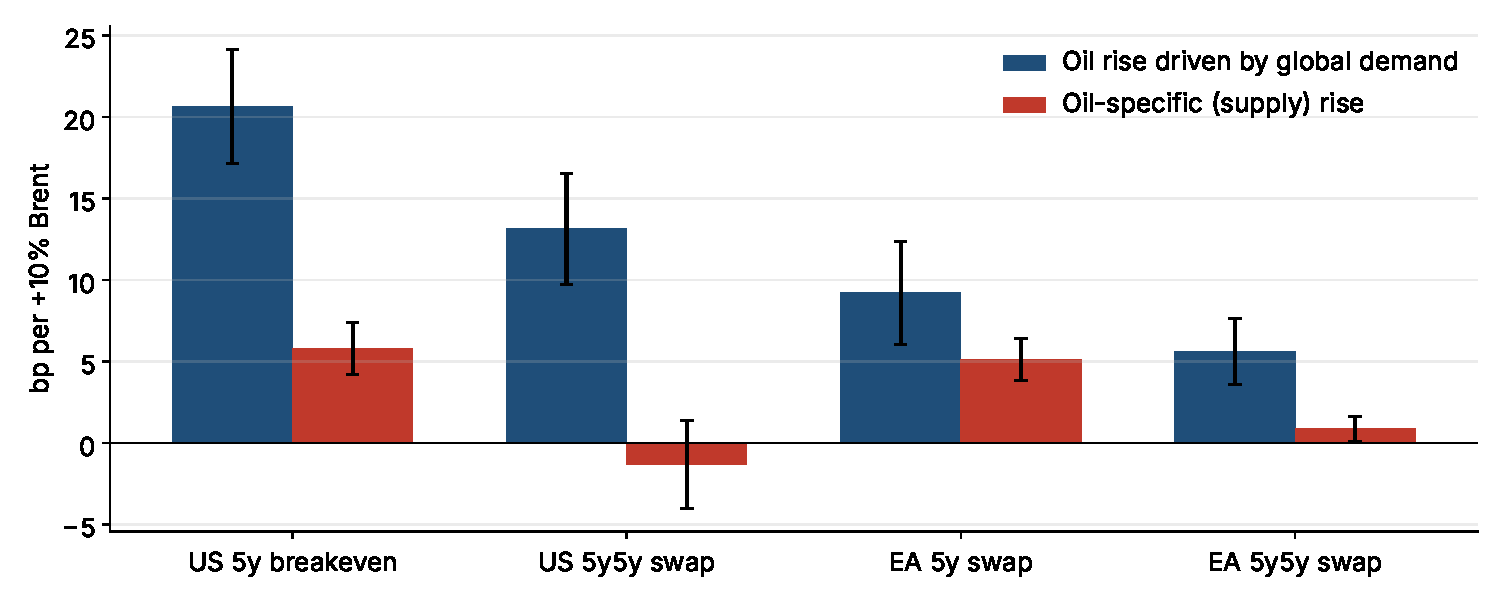
\includegraphics[width=0.92\textwidth]{fig08_market_by_shock_type.pdf}
\caption{Response of inflation compensation to a 10\% Brent rise, by type of shock (weekly, 2004--2026, 90\% confidence intervals).}\label{fig:shockmkt}
\end{figure}

Realized inflation confirms this reading (Figure~\ref{fig:shockinfl}, Table~\ref{tab:inflshock} in the Appendix). After an oil-specific shock, headline inflation rises by about 0.3 pp within three to six months and returns to zero within about a year, with little effect on core. After a demand-driven rise, the effect is larger and persistent, reaching about 1 pp on headline and 0.4 pp on core after 12--24 months. These larger effects capture the demand expansion as a whole, not the effect of oil alone. The interpretation is consistent with the cash-flow versus discount-rate distinction: an oil-specific shock is a temporary cost shock, which markets expect central banks to look through, whereas a demand-driven oil rise signals a stronger and more inflationary economy, and therefore changes the long-term outlook.

\begin{figure}[!htbp]
\centering
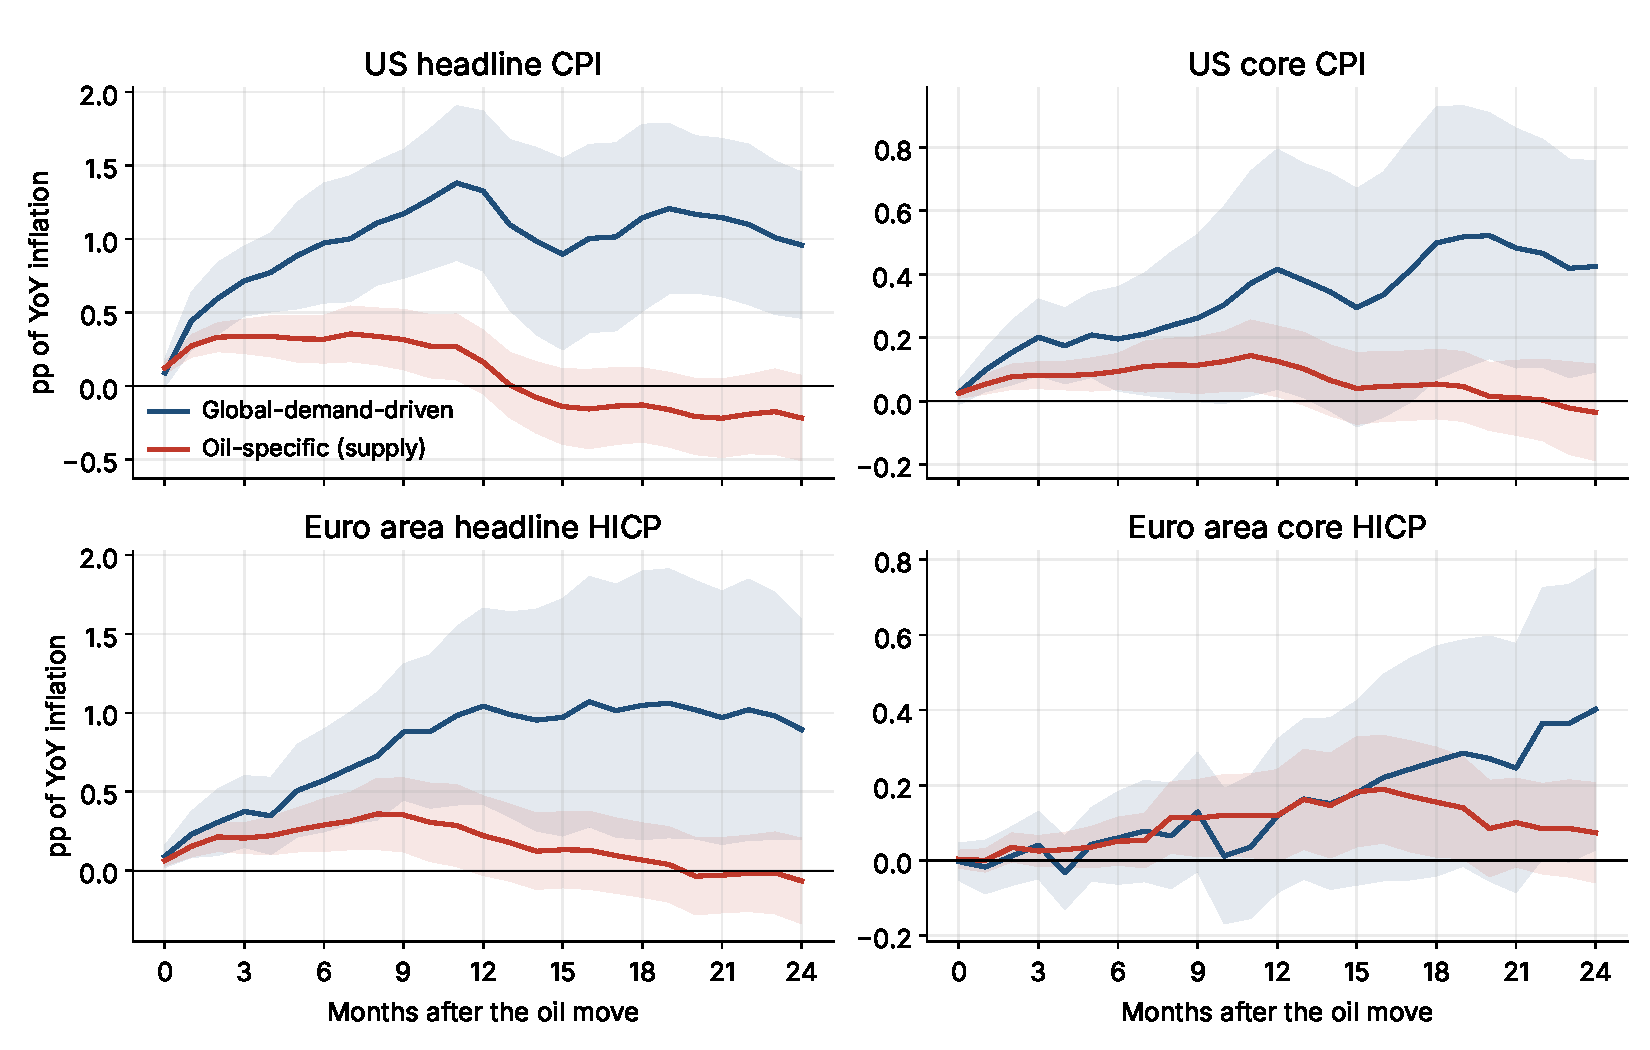
\includegraphics[width=\figwidth]{fig09_inflation_by_shock_type.pdf}
\caption{Response of YoY inflation to a 10\% Brent rise, by type of shock (2005--2026, 90\% bands).}\label{fig:shockinfl}
\end{figure}

\subsection{Out-of-sample test: the 2026 oil shock}

Figure~\ref{fig:oos} and Table~\ref{tab:oos} report the out-of-sample test. The model estimated on 1990--2019 predicts US headline inflation of 3.76\% in September 2026, against an actual 3.7\%. It also captures the peak of 4.3\% in May (actual 4.2\%), and every monthly observation lies inside the 90\% band. The root mean squared error is 0.21 pp, against 0.88 pp for the no-shock counterfactual. Oil explains about 1.1 pp of US headline inflation by September, and 1.3 pp at the peak. US and euro area core inflation are also well predicted, with an oil contribution of only 0--0.3 pp.

\begin{figure}[!htbp]
\centering
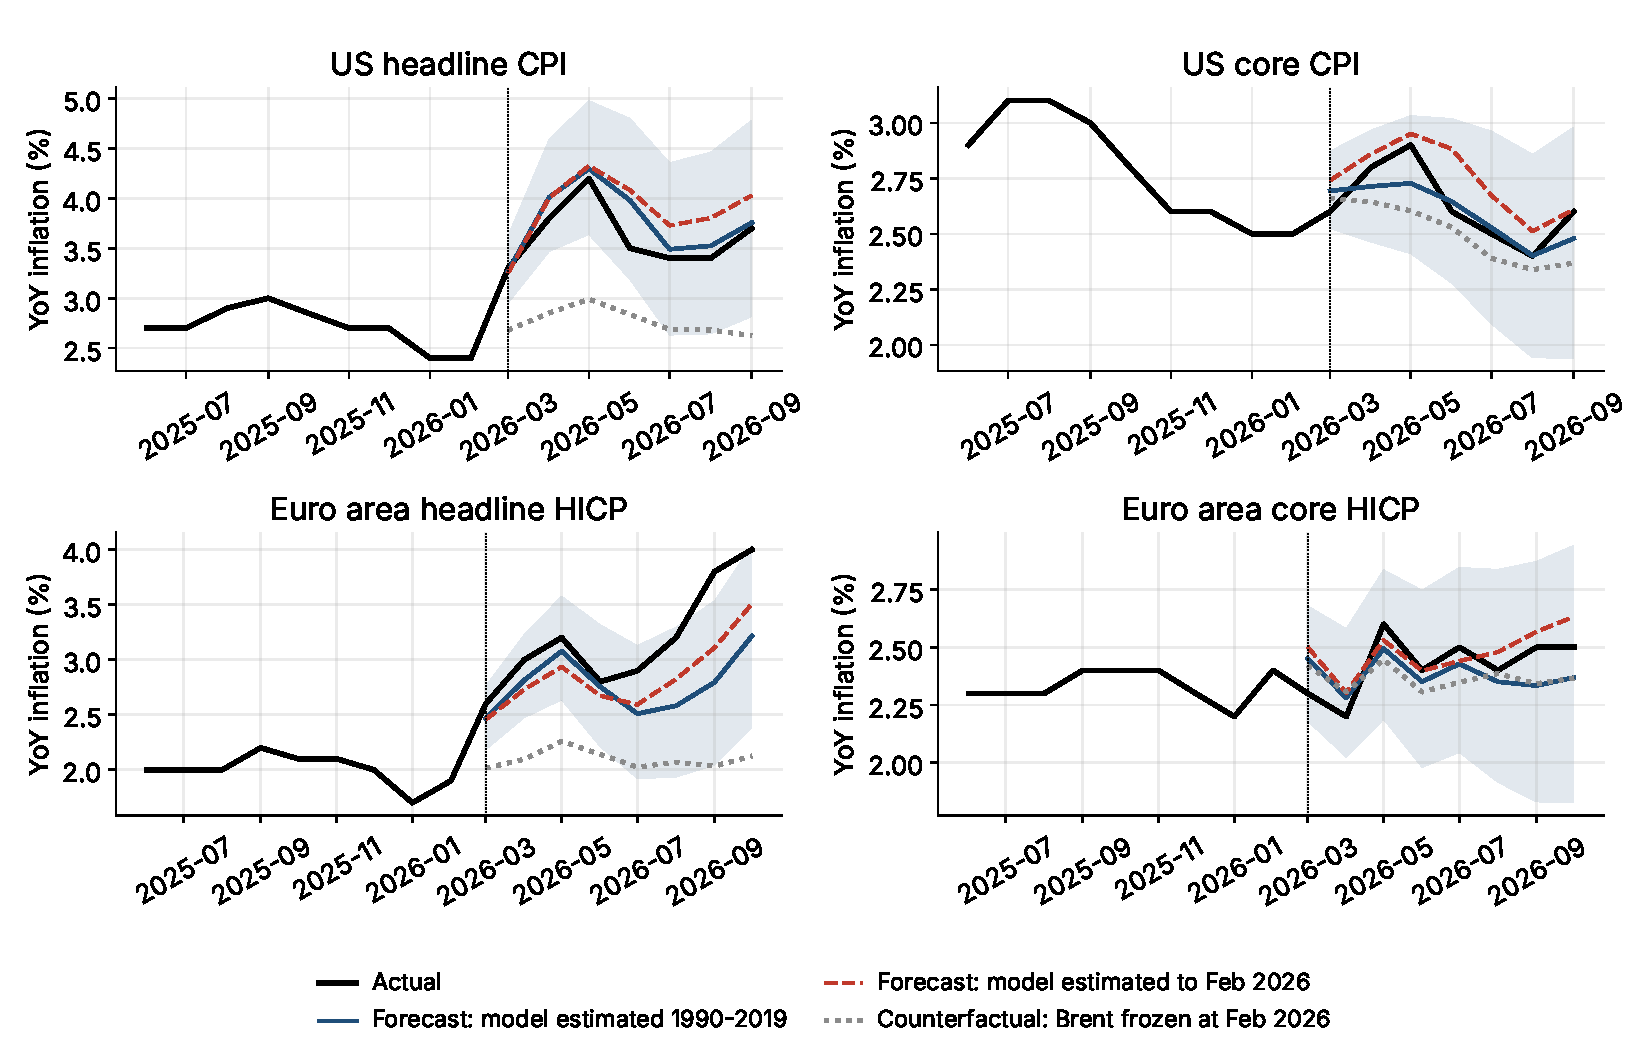
\includegraphics[width=\figwidth]{fig06_out_of_sample_2026.pdf}
\caption{Out-of-sample forecasts of inflation after the March 2026 oil shock. Models of equation~(\ref{eq:ardl}) estimated on 1990--2019 (solid, with 90\% band) and on 1990--February 2026 (dashed), simulated with the actual Brent path. The dotted line freezes Brent at its February 2026 level.}\label{fig:oos}
\end{figure}

\begin{table}[!htbp]
\centering\small
\caption{Out-of-sample forecasts after the March 2026 oil shock}\label{tab:oos}
\begin{minipage}{\textwidth}\centering
\resizebox{\textwidth}{!}{\begin{tabular}{llrrrrrrr}
\toprule
 & Estimation & Actual & Forecast & No-shock & Oil & RMSE & RMSE & In 90\%\\
Series & sample & (end) & (end) & (end) & contrib. & model & no-shock & band\\
\midrule
US headline CPI & 1990--2019 & 3.7 & 3.76 & 2.62 & 1.13 & 0.21 & 0.88 & 100\%\\
 & 1990--Feb 2026 & 3.7 & 4.03 & 2.72 & 1.31 & 0.33 & 0.83 & --\\
\addlinespace
US core CPI & 1990--2019 & 2.6 & 2.48 & 2.37 & 0.11 & 0.10 & 0.17 & 100\%\\
 & 1990--Feb 2026 & 2.6 & 2.61 & 2.33 & 0.28 & 0.14 & 0.14 & --\\
\addlinespace
Euro area headline HICP & 1990--2019 & 4.0 & 3.21 & 2.13 & 1.09 & 0.53 & 1.18 & 88\%\\
 & 1990--Feb 2026 & 4.0 & 3.50 & 2.15 & 1.36 & 0.38 & 1.22 & --\\
\addlinespace
Euro area core HICP & 1990--2019 & 2.5 & 2.37 & 2.37 & 0.00 & 0.11 & 0.12 & 100\%\\
 & 1990--Feb 2026 & 2.5 & 2.63 & 2.41 & 0.22 & 0.10 & 0.11 & --\\
\bottomrule
\end{tabular}}
\par\smallskip{\footnotesize\raggedright \textit{Notes:} Inflation in \%; forecast end is September 2026 (US) and October 2026 (euro area). ``No-shock'' freezes Brent at its February 2026 level; ``Oil contrib.'' is the difference between forecast and no-shock path at the end. RMSE over March 2026 to the forecast end. The 90\% band is computed for the 1990--2019 model.\par}
\end{minipage}
\end{table}

Two results stand out. First, the model estimated before 2020 forecasts US inflation better than the model that includes 2021--23 (RMSE 0.21 versus 0.33 pp). The 2026 shock thus behaved like the pre-2020 regime: a strong but transitory effect on headline inflation and almost none on core. This matches the markets' decision to leave long-term expectations unchanged in 2026. Second, the model under-predicts euro area headline inflation at the end of the period (3.2--3.5\% predicted versus 4.0\% actual in October). Gas prices and the exchange rate, which are not in our model, are the most likely explanations.

\subsection{State dependence and asymmetry}

Figure~\ref{fig:reg} and Table~\ref{tab:regime} examine two refinements. When inflation in the previous month exceeded 3\%, headline pass-through is roughly twice as fast: 0.68 pp after six months in the US against 0.36 pp in normal times, and 0.85 against 0.26 pp in the euro area. Core pass-through, however, does not differ significantly across regimes, so the larger post-2020 core response is not explained by the inflation regime alone. Estimates for the euro area high-inflation regime rest on only 40 months and are imprecise.

Oil price rises pass through more persistently than falls, especially in the euro area, where a 10\% rise adds 0.85 pp to headline inflation after a year and a 10\% fall subtracts only 0.23 pp. This is consistent with the asymmetric adjustment of retail prices \citep{peltzman2000}. Market expectations, in contrast, respond symmetrically to rises and falls and show no significant regime dependence (Table~\ref{tab:regmkt}). Markets do not appear to price the asymmetry seen in realized inflation, although the confidence bands are wide.

\begin{figure}[!htbp]
\centering
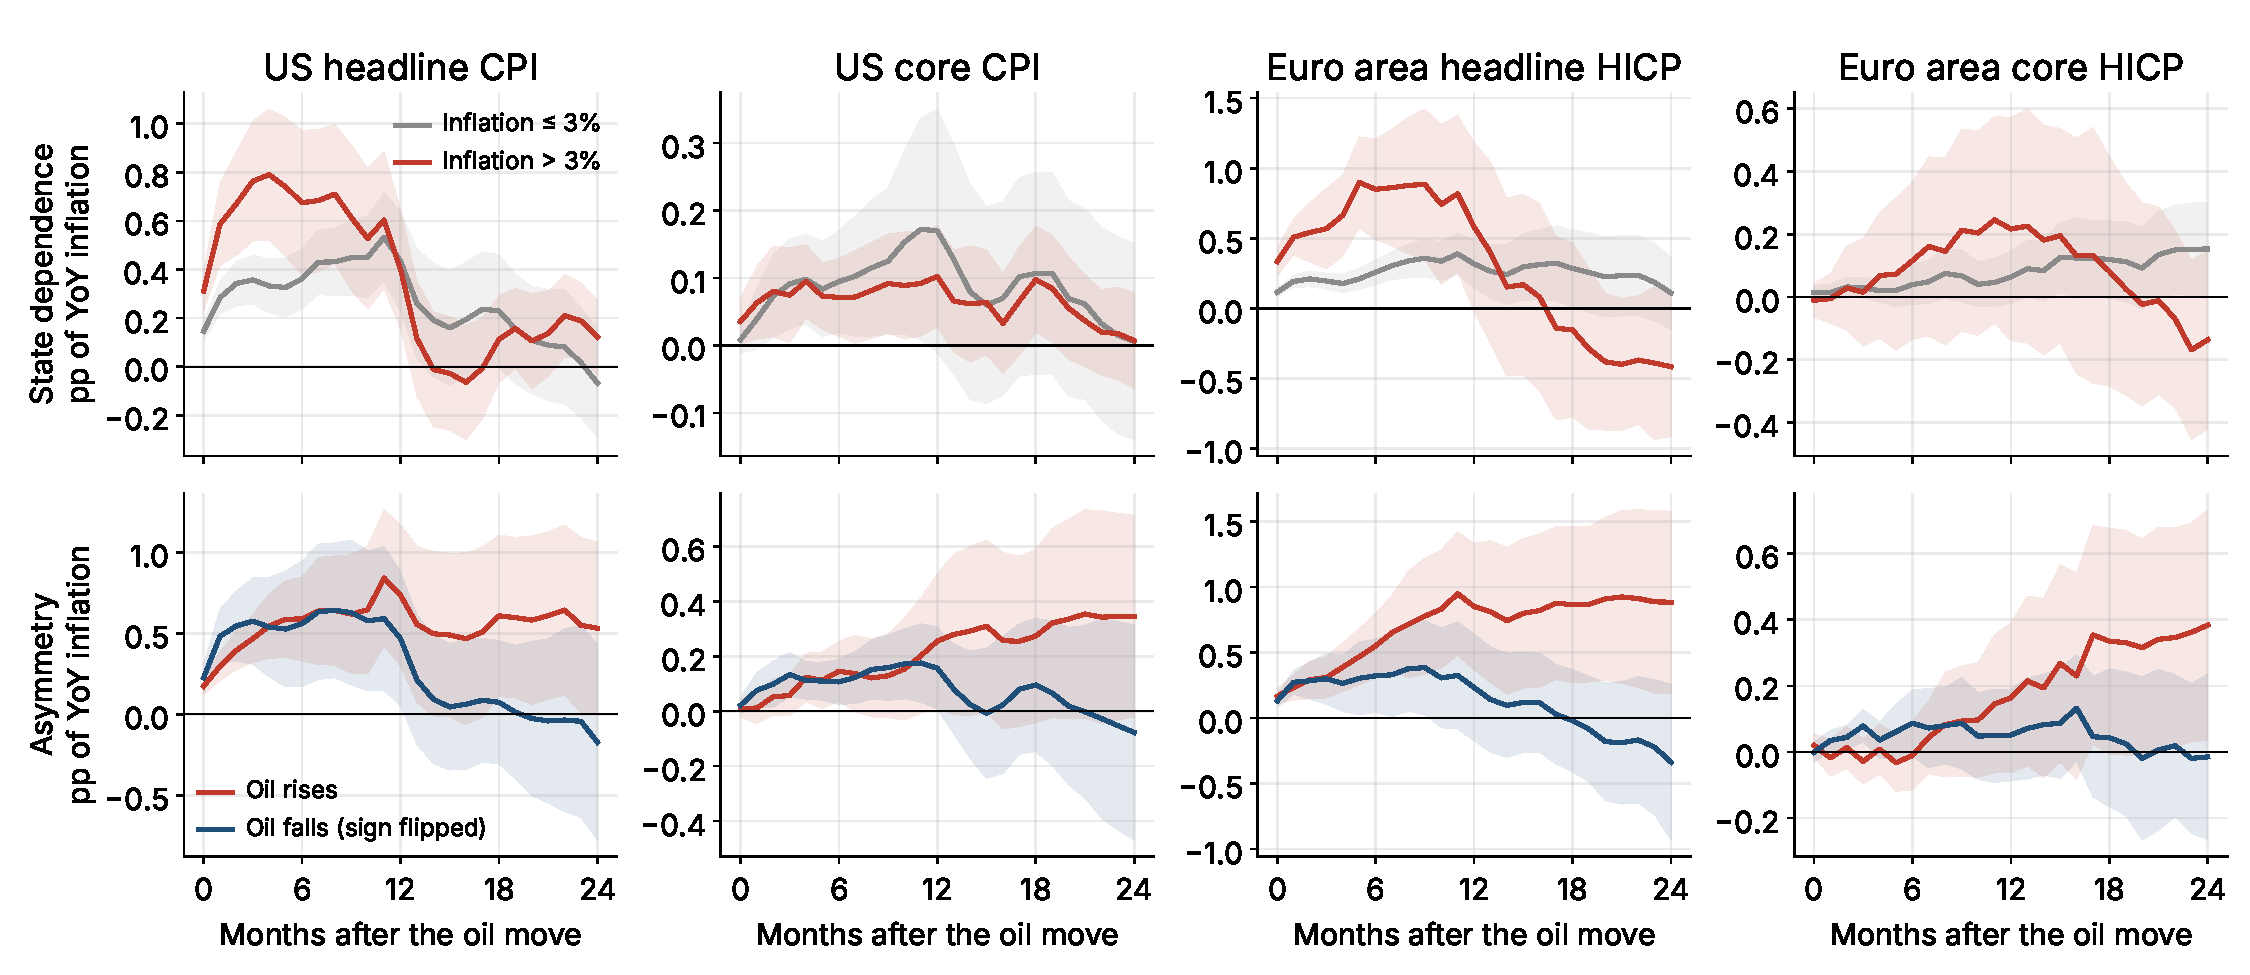
\includegraphics[width=\figwidth]{fig10_regime_and_asymmetry.pdf}
\caption{State dependence (top: previous month's headline inflation above or below 3\%) and asymmetry (bottom: oil rises versus falls, the latter with sign flipped). Responses to a 10\% Brent move, 90\% bands.}\label{fig:reg}
\end{figure}

\subsection{Robustness}

Table~\ref{tab:rob} shows that the pass-through estimates are robust. Using month-end rather than average Brent prices lowers the estimates by about a quarter, as expected from the timing mismatch with monthly average consumer prices. WTI gives the same results as month-end Brent. The number of lags in the controls hardly matters, and the distributed-lag model (the cumulative-sum-of-coefficients approach) gives somewhat smaller estimates, similar to those obtained with month-end prices. Excluding the 2008--09 crisis and 2020 lowers the headline estimates by about a quarter (and core estimates by somewhat more), so these large episodes contribute to identification. The broad commodity index gives larger effects per 10\% move only because it is less volatile than oil. On the market side (Table~\ref{tab:robmkt}), daily, weekly and monthly estimates lead to the same conclusions: 5-year expectations react significantly, and the 5y5y response is small (between $-0.4$ and $2.4$ bp).

\section{Conclusion}

Table~\ref{tab:hyp} summarizes the evidence on our hypotheses. A 10\% oil price shock adds about 0.4--0.55 pp to headline inflation within 6--12 months in the US and the euro area, but only 0.1--0.2 pp to core inflation. Pass-through is larger in the US than in the euro area over the full sample, contrary to our initial hypothesis, and pass-through to core has risen markedly since 2020. Markets price oil into 5-year inflation expectations but, on average, not into the 5y5y forward, except in 2021--23.

\begin{table}[!htbp]
\centering\small
\caption{Summary of the evidence}\label{tab:hyp}
\begin{tabular}{p{6.2cm}p{1.9cm}p{6.4cm}}
\toprule
Hypothesis & Verdict & Main evidence\\
\midrule
H1: Strong, fast pass-through to headline; weak, lagged to core & Supported & Headline +0.55 pp (US), +0.42 pp (EA) at 6 months; core +0.12 / +0.05 pp\\
H2: Stronger pass-through in the euro area & Rejected (full sample) & US larger before 2020; EA larger since 2020 (gas, euro)\\
H3: Short-term expectations react, 5y5y does not & Supported, with exceptions & 5y: +5--7 bp; 5y5y $\approx$ 0 except 2021--23; 5y5y moves with demand-driven, not oil-specific, shocks\\
H4: Pass-through has changed over time & Supported & Core pass-through $\approx$ 0 before 2020, 0.4--0.7 pp since; 2026 shock behaved like the pre-2020 regime\\
\bottomrule
\end{tabular}
\end{table}

Two results go beyond the initial hypotheses. First, the market reaction depends on why oil moves: oil-specific shocks leave long-term expectations anchored, while demand-driven oil rises move them. Second, a model estimated only on pre-2020 data accurately predicts US inflation after the record oil shock of March 2026. This suggests that markets were right to treat that shock as temporary.

\paragraph{Limitations.} Oil prices are not fully exogenous: global demand moves both oil and inflation. Our sign and narrative restrictions address this only partially, and the stock-based identification may misclassify some demand-driven episodes. Identified oil supply news shocks \citep{kanzig2021} would provide an independent check. Breakeven inflation and inflation swaps contain inflation risk and liquidity premia \citep{damico2018}, which may co-move with oil and equity prices. The post-2020 sample is short and dominated by a few large episodes. Finally, for the euro area our analysis omits natural gas prices and the EUR/USD exchange rate, which likely explains part of the larger post-2020 pass-through and the out-of-sample forecast error in 2026.

\begin{thebibliography}{99}
\setlength{\itemsep}{0.15em}\small

\bibitem[Antol\'{i}n-D\'{i}az and Rubio-Ram\'{i}rez(2018)]{antolin2018}
Antol\'{i}n-D\'{i}az, J. and Rubio-Ram\'{i}rez, J.~F. (2018). Narrative sign restrictions for SVARs. \textit{American Economic Review}, 108(10), 2802--2829.

\bibitem[Baumeister and Hamilton(2019)]{baumeister2019}
Baumeister, C. and Hamilton, J.~D. (2019). Structural interpretation of vector autoregressions with incomplete identification: Revisiting the role of oil supply and demand shocks. \textit{American Economic Review}, 109(5), 1873--1910.

\bibitem[Blanchard and Gal\'{i}(2010)]{blanchard2010}
Blanchard, O.~J. and Gal\'{i}, J. (2010). The macroeconomic effects of oil price shocks: Why are the 2000s so different from the 1970s? In J.~Gal\'{i} and M.~Gertler (eds.), \textit{International Dimensions of Monetary Policy}, 373--421. University of Chicago Press.

\bibitem[Coibion and Gorodnichenko(2015)]{coibion2015}
Coibion, O. and Gorodnichenko, Y. (2015). Is the Phillips curve alive and well after all? Inflation expectations and the missing disinflation. \textit{American Economic Journal: Macroeconomics}, 7(1), 197--232.

\bibitem[D'Amico et~al.(2018)]{damico2018}
D'Amico, S., Kim, D.~H. and Wei, M. (2018). Tips from TIPS: The informational content of Treasury Inflation-Protected Security prices. \textit{Journal of Financial and Quantitative Analysis}, 53(1), 395--436.

\bibitem[G\"{u}rkaynak et~al.(2005)]{gurkaynak2005}
G\"{u}rkaynak, R.~S., Sack, B. and Swanson, E. (2005). The sensitivity of long-term interest rates to economic news: Evidence and implications for macroeconomic models. \textit{American Economic Review}, 95(1), 425--436.

\bibitem[Hooker(2002)]{hooker2002}
Hooker, M.~A. (2002). Are oil shocks inflationary? Asymmetric and nonlinear specifications versus changes in regime. \textit{Journal of Money, Credit and Banking}, 34(2), 540--561.

\bibitem[Jord\`{a}(2005)]{jorda2005}
Jord\`{a}, \`{O}. (2005). Estimation and inference of impulse responses by local projections. \textit{American Economic Review}, 95(1), 161--182.

\bibitem[K\"{a}nzig(2021)]{kanzig2021}
K\"{a}nzig, D.~R. (2021). The macroeconomic effects of oil supply news: Evidence from OPEC announcements. \textit{American Economic Review}, 111(4), 1092--1125.

\bibitem[Kilian(2009)]{kilian2009}
Kilian, L. (2009). Not all oil price shocks are alike: Disentangling demand and supply shocks in the crude oil market. \textit{American Economic Review}, 99(3), 1053--1069.

\bibitem[Kilian and Park(2009)]{kilianpark2009}
Kilian, L. and Park, C. (2009). The impact of oil price shocks on the U.S. stock market. \textit{International Economic Review}, 50(4), 1267--1287.

\bibitem[Kilian and Zhou(2022)]{kilianzhou2022}
Kilian, L. and Zhou, X. (2022). Oil prices, gasoline prices, and inflation expectations. \textit{Journal of Applied Econometrics}, 37(5), 867--881.

\bibitem[Mork(1989)]{mork1989}
Mork, K.~A. (1989). Oil and the macroeconomy when prices go up and down: An extension of Hamilton's results. \textit{Journal of Political Economy}, 97(3), 740--744.

\bibitem[Newey and West(1987)]{newey1987}
Newey, W.~K. and West, K.~D. (1987). A simple, positive semi-definite, heteroskedasticity and autocorrelation consistent covariance matrix. \textit{Econometrica}, 55(3), 703--708.

\bibitem[Peltzman(2000)]{peltzman2000}
Peltzman, S. (2000). Prices rise faster than they fall. \textit{Journal of Political Economy}, 108(3), 466--502.

\bibitem[Ready(2018)]{ready2018}
Ready, R.~C. (2018). Oil prices and the stock market. \textit{Review of Finance}, 22(1), 155--176.

\bibitem[Reuters(2026)]{reuters2026}
Reuters (2026). Brent heads for record monthly jump as Iran conflict widens. 30 March 2026. Reported by \textit{Profit (Pakistan Today)}, \url{https://profit.pakistantoday.com.pk/2026/03/30/brent-heads-for-record-monthly-jump-as-iran-conflict-widens}.

\bibitem[Uhlig(2005)]{uhlig2005}
Uhlig, H. (2005). What are the effects of monetary policy on output? Results from an agnostic identification procedure. \textit{Journal of Monetary Economics}, 52(2), 381--419.

\end{thebibliography}

\clearpage
\appendix
\section{Additional results}

\begin{figure}[!htbp]
\centering
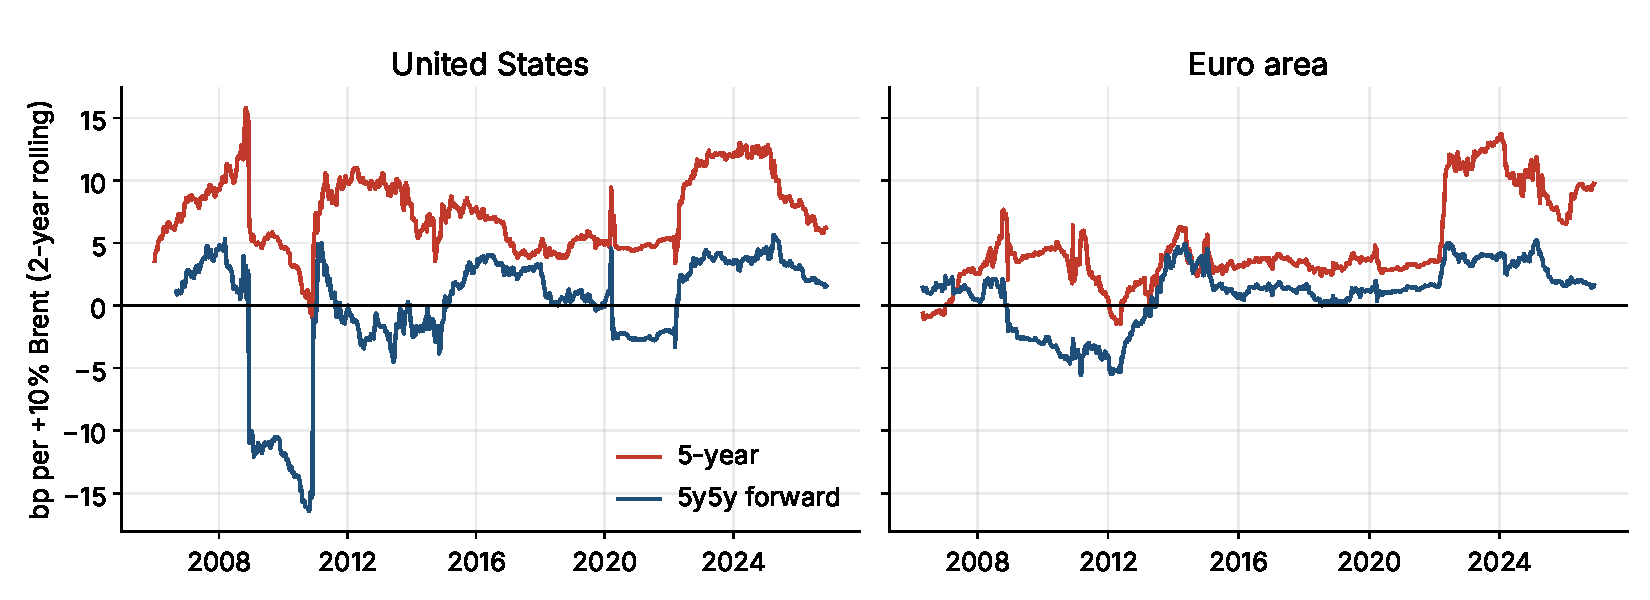
\includegraphics[width=\figwidth]{fig03_rolling_market_betas.pdf}
\caption{Rolling two-year sensitivity of 5-year and 5y5y inflation compensation to a 10\% Brent move (weekly, S\&P 500 control).}\label{fig:roll}
\end{figure}

\begin{table}[!htbp]
\centering\small
\caption{Inflation response by type of oil shock (pp per 10\% Brent move, 2005--2026)}\label{tab:inflshock}
\begin{tabular}{lrrrrr}
\toprule
 & \multicolumn{5}{c}{Months after the oil move ($h$)}\\ \cmidrule(lr){2-6}
 & 3 & 6 & 12 & 18 & 24\\
\midrule
\multicolumn{6}{l}{\textit{US headline CPI}}\\
\quad Global-demand-driven & 0.71 & 0.97 & 1.33 & 1.15 & 0.96\\
\quad Oil-specific (supply) & 0.34 & 0.32 & 0.16 & $-$0.13 & $-$0.22\\
\quad All oil moves & 0.42 & 0.46 & 0.45 & 0.20 & 0.09\\
\addlinespace
\multicolumn{6}{l}{\textit{US core CPI}}\\
\quad Global-demand-driven & 0.20 & 0.20 & 0.42 & 0.50 & 0.42\\
\quad Oil-specific (supply) & 0.08 & 0.09 & 0.13 & 0.05 & $-$0.04\\
\quad All oil moves & 0.11 & 0.12 & 0.20 & 0.17 & 0.09\\
\addlinespace
\multicolumn{6}{l}{\textit{Euro area headline HICP}}\\
\quad Global-demand-driven & 0.38 & 0.57 & 1.04 & 1.05 & 0.89\\
\quad Oil-specific (supply) & 0.21 & 0.29 & 0.22 & 0.07 & $-$0.07\\
\quad All oil moves & 0.24 & 0.35 & 0.41 & 0.31 & 0.18\\
\addlinespace
\multicolumn{6}{l}{\textit{Euro area core HICP}}\\
\quad Global-demand-driven & 0.04 & 0.06 & 0.12 & 0.27 & 0.40\\
\quad Oil-specific (supply) & 0.03 & 0.05 & 0.12 & 0.15 & 0.07\\
\quad All oil moves & 0.03 & 0.06 & 0.12 & 0.18 & 0.15\\
\bottomrule
\end{tabular}
\end{table}

\begin{table}[!htbp]
\centering\small
\caption{State dependence and asymmetry of inflation pass-through (pp per 10\% Brent move)}\label{tab:regime}
\begin{minipage}{\textwidth}\centering
\resizebox{\textwidth}{!}{\begin{tabular}{lrrrrrrrr}
\toprule
 & \multicolumn{2}{c}{Inflation $\leq$ 3\%} & \multicolumn{2}{c}{Inflation $>$ 3\%} & \multicolumn{2}{c}{Oil rise} & \multicolumn{2}{c}{Oil fall (flipped)}\\
\cmidrule(lr){2-3}\cmidrule(lr){4-5}\cmidrule(lr){6-7}\cmidrule(lr){8-9}
 & $h=6$ & $h=12$ & $h=6$ & $h=12$ & $h=6$ & $h=12$ & $h=6$ & $h=12$\\
\midrule
US headline CPI & 0.36 & 0.43 & 0.68 & 0.40 & 0.59 & 0.73 & 0.56 & 0.47\\
US core CPI & 0.10 & 0.17 & 0.07 & 0.10 & 0.14 & 0.26 & 0.11 & 0.16\\
Euro area headline HICP & 0.26 & 0.32 & 0.85 & 0.58 & 0.55 & 0.85 & 0.32 & 0.23\\
Euro area core HICP & 0.04 & 0.06 & 0.12 & 0.22 & $-$0.01 & 0.16 & 0.09 & 0.05\\
\bottomrule
\end{tabular}}
\par\smallskip{\footnotesize\raggedright \textit{Notes:} Regime defined by own-region headline inflation in the previous month. ``Oil fall'' reports the response to the negative part of the oil return, so a positive value means that a 10\% fall lowers inflation by that amount.\par}
\end{minipage}
\end{table}

\begin{table}[!htbp]
\centering\small
\caption{Market sensitivity by inflation regime and by direction of the oil move (bp per 10\% Brent move, weekly)}\label{tab:regmkt}
\begin{minipage}{\textwidth}\centering
\begin{tabular}{lrrrr}
\toprule
 & Inflation $\leq$ 3\% & Inflation $>$ 3\% & Oil up & Oil down\\
\midrule
US 5y breakeven & $5.99^{***}$ & $8.34^{***}$ & $5.31^{***}$ & $8.19^{***}$\\
 & {\footnotesize (0.76)} & {\footnotesize (2.57)} & {\footnotesize (0.85)} & {\footnotesize (1.71)}\\
US 5y5y swap & $0.62$ & $-2.21$ & $1.61$ & $-2.21$\\
 & {\footnotesize (0.95)} & {\footnotesize (3.42)} & {\footnotesize (1.30)} & {\footnotesize (2.96)}\\
Euro area 5y swap & $4.76^{***}$ & $7.45^{***}$ & $5.83^{***}$ & $4.99^{***}$\\
 & {\footnotesize (0.64)} & {\footnotesize (2.58)} & {\footnotesize (1.42)} & {\footnotesize (1.38)}\\
Euro area 5y5y swap & $1.49^{***}$ & $0.23$ & $1.38^{*}$ & $0.98$\\
 & {\footnotesize (0.33)} & {\footnotesize (1.53)} & {\footnotesize (0.75)} & {\footnotesize (0.82)}\\
\bottomrule
\end{tabular}
\par\smallskip{\footnotesize\raggedright \textit{Notes:} Regime defined by headline inflation two months earlier, i.e.\ the latest figure known to investors. S\&P 500 control included. Newey--West standard errors in parentheses.\par}
\end{minipage}
\end{table}

\begin{table}[!htbp]
\centering\small
\caption{Robustness of pass-through estimates (pp per 10\% oil move)}\label{tab:rob}
\begin{minipage}{\textwidth}\centering
\resizebox{\textwidth}{!}{\begin{tabular}{lrrrrrrrr}
\toprule
 & \multicolumn{2}{c}{US headline} & \multicolumn{2}{c}{US core} & \multicolumn{2}{c}{EA headline} & \multicolumn{2}{c}{EA core}\\
\cmidrule(lr){2-3}\cmidrule(lr){4-5}\cmidrule(lr){6-7}\cmidrule(lr){8-9}
Specification & $h=6$ & $h=12$ & $h=6$ & $h=12$ & $h=6$ & $h=12$ & $h=6$ & $h=12$\\
\midrule
Baseline (avg Brent, 6 lags) & 0.55 & 0.55 & 0.12 & 0.19 & 0.41 & 0.49 & 0.05 & 0.11\\
\midrule
Month-end Brent & 0.40 & 0.44 & 0.09 & 0.15 & 0.30 & 0.38 & 0.03 & 0.08\\
Month-end WTI & 0.39 & 0.42 & 0.09 & 0.15 & 0.27 & 0.34 & 0.02 & 0.07\\
Broad commodities (BCOM) & 1.03 & 1.23 & 0.18 & 0.32 & 0.72 & 0.94 & 0.09 & 0.23\\
3 lags of controls & 0.53 & 0.54 & 0.11 & 0.18 & 0.41 & 0.50 & 0.04 & 0.10\\
12 lags of controls & 0.55 & 0.56 & 0.12 & 0.20 & 0.42 & 0.50 & 0.05 & 0.13\\
Excluding 2008--09 crisis and 2020 & 0.41 & 0.43 & 0.08 & 0.14 & 0.32 & 0.37 & 0.01 & 0.07\\
Sample 2004--2026 & 0.60 & 0.56 & 0.13 & 0.21 & 0.47 & 0.52 & 0.07 & 0.14\\
Distributed-lag model (ARDL), 1990--Feb 2026 & 0.43 & 0.41 & 0.10 & 0.15 & 0.32 & 0.38 & 0.05 & 0.09\\
\bottomrule
\end{tabular}}
\par\smallskip{\footnotesize\raggedright \textit{Notes:} Local projections as in equation~(\ref{eq:lp}) unless stated. ``Distributed-lag model'' reports the cumulative dynamic multiplier from equation~(\ref{eq:ardl}).\par}
\end{minipage}
\end{table}

\begin{table}[!htbp]
\centering\small
\caption{Robustness of market sensitivities to data frequency (bp per 10\% Brent move)}\label{tab:robmkt}
\begin{minipage}{\textwidth}\centering
\begin{tabular}{lrrrr}
\toprule
 & Daily & Daily & Weekly & Monthly\\
 & (same day) & ($t-1$ to $t+1$) & (baseline) & \\
\midrule
US 5y breakeven & 6.42 & $8.31^{***}$ & $6.80^{***}$ & $9.71^{***}$\\
 & & {\footnotesize (0.62)} & {\footnotesize (0.96)} & {\footnotesize (1.17)}\\
US 5y5y swap & 0.99 & $2.40^{***}$ & $-0.37$ & $1.25$\\
 & & {\footnotesize (0.80)} & {\footnotesize (1.51)} & {\footnotesize (0.87)}\\
Euro area 5y swap & 3.79 & $6.00^{***}$ & $5.40^{***}$ & $7.78^{***}$\\
 & & {\footnotesize (0.55)} & {\footnotesize (0.75)} & {\footnotesize (0.97)}\\
Euro area 5y5y swap & 1.29 & $1.94^{***}$ & $1.17^{**}$ & $2.03^{***}$\\
 & & {\footnotesize (0.40)} & {\footnotesize (0.46)} & {\footnotesize (0.41)}\\
\bottomrule
\end{tabular}
\par\smallskip{\footnotesize\raggedright \textit{Notes:} S\&P 500 control included. ``Daily ($t-1$ to $t+1$)'' sums the coefficients on the previous, same-day and next-day oil return to account for different market closing times.\par}
\end{minipage}
\end{table}

\paragraph{Replication.} All results, tables and figures are produced from the Bloomberg download file by\\ \texttt{code/oil\_passthrough\_analysis.py}; the tables are converted to \LaTeX{} by \texttt{code/make\_tables.py}. Run \texttt{run\_all.sh} to rebuild everything.

\end{document}
